\documentclass[11pt]{article}
\newcommand{\ListaTitulo}{Lista 01: Tipos de variável, tabelas e gráficos}
% Preâmbulo compartilhado: MATF14, Listas de Exercícios 2026
% Usado por ListaNN.tex e GabaritoNN.tex via % Preâmbulo compartilhado: MATF14, Listas de Exercícios 2026
% Usado por ListaNN.tex e GabaritoNN.tex via % Preâmbulo compartilhado: MATF14, Listas de Exercícios 2026
% Usado por ListaNN.tex e GabaritoNN.tex via \input{preamble}

\usepackage[utf8]{inputenc}
\usepackage[T1]{fontenc}
\usepackage[brazil]{babel}
\usepackage{fullpage}
\usepackage{amsmath,amssymb}
\usepackage{enumitem}
\usepackage{xcolor}
\usepackage{fancyhdr}
\usepackage{titlesec}
\usepackage{listings}
\usepackage{hyperref}
\usepackage{booktabs}
\usepackage{graphicx}
\usepackage{tikz}

\definecolor{matf14azul}{HTML}{0D3B54}
\definecolor{matf14dourado}{HTML}{C9971E}

\titleformat{\section}{\normalfont\Large\bfseries\color{matf14azul}}{\thesection}{1em}{}
\titleformat{\subsection}{\normalfont\large\bfseries\color{matf14azul}}{\thesubsection}{1em}{}

\providecommand{\ListaTitulo}{Lista de Exercícios}

\setlength{\headheight}{14pt}
\pagestyle{fancy}
\fancyhf{}
\lhead{\small MATF14: Estatística Econômica I}
\rhead{\small \ListaTitulo}
\cfoot{\thepage}
\renewcommand{\headrulewidth}{0.4pt}

\lstset{
  basicstyle=\ttfamily\small,
  breaklines=true,
  frame=single,
  columns=fullflexible,
  backgroundcolor=\color{gray!8},
  commentstyle=\color{matf14dourado},
  keywordstyle=\color{matf14azul}\bfseries,
  language=R
}

\newcounter{questaocounter}
\newenvironment{questao}[1]{%
  \stepcounter{questaocounter}%
  \bigskip\noindent\textbf{Questão #1.}\ %
}{\par}

\newcommand{\cabecalho}[2]{%
  \begin{center}
    {\Large\bfseries\color{matf14azul} #1}\\[0.3em]
    {\large #2}
  \end{center}
  \vspace{0.5em}
  \noindent\rule{\linewidth}{0.6pt}
  \vspace{0.5em}
}

\newenvironment{solucao}{%
  \par\smallskip\noindent\textit{\color{matf14dourado!80!black}Solução.}\ %
}{\hfill$\blacksquare$\par}


\usepackage[utf8]{inputenc}
\usepackage[T1]{fontenc}
\usepackage[brazil]{babel}
\usepackage{fullpage}
\usepackage{amsmath,amssymb}
\usepackage{enumitem}
\usepackage{xcolor}
\usepackage{fancyhdr}
\usepackage{titlesec}
\usepackage{listings}
\usepackage{hyperref}
\usepackage{booktabs}
\usepackage{graphicx}
\usepackage{tikz}

\definecolor{matf14azul}{HTML}{0D3B54}
\definecolor{matf14dourado}{HTML}{C9971E}

\titleformat{\section}{\normalfont\Large\bfseries\color{matf14azul}}{\thesection}{1em}{}
\titleformat{\subsection}{\normalfont\large\bfseries\color{matf14azul}}{\thesubsection}{1em}{}

\providecommand{\ListaTitulo}{Lista de Exercícios}

\setlength{\headheight}{14pt}
\pagestyle{fancy}
\fancyhf{}
\lhead{\small MATF14: Estatística Econômica I}
\rhead{\small \ListaTitulo}
\cfoot{\thepage}
\renewcommand{\headrulewidth}{0.4pt}

\lstset{
  basicstyle=\ttfamily\small,
  breaklines=true,
  frame=single,
  columns=fullflexible,
  backgroundcolor=\color{gray!8},
  commentstyle=\color{matf14dourado},
  keywordstyle=\color{matf14azul}\bfseries,
  language=R
}

\newcounter{questaocounter}
\newenvironment{questao}[1]{%
  \stepcounter{questaocounter}%
  \bigskip\noindent\textbf{Questão #1.}\ %
}{\par}

\newcommand{\cabecalho}[2]{%
  \begin{center}
    {\Large\bfseries\color{matf14azul} #1}\\[0.3em]
    {\large #2}
  \end{center}
  \vspace{0.5em}
  \noindent\rule{\linewidth}{0.6pt}
  \vspace{0.5em}
}

\newenvironment{solucao}{%
  \par\smallskip\noindent\textit{\color{matf14dourado!80!black}Solução.}\ %
}{\hfill$\blacksquare$\par}


\usepackage[utf8]{inputenc}
\usepackage[T1]{fontenc}
\usepackage[brazil]{babel}
\usepackage{fullpage}
\usepackage{amsmath,amssymb}
\usepackage{enumitem}
\usepackage{xcolor}
\usepackage{fancyhdr}
\usepackage{titlesec}
\usepackage{listings}
\usepackage{hyperref}
\usepackage{booktabs}
\usepackage{graphicx}
\usepackage{tikz}

\definecolor{matf14azul}{HTML}{0D3B54}
\definecolor{matf14dourado}{HTML}{C9971E}

\titleformat{\section}{\normalfont\Large\bfseries\color{matf14azul}}{\thesection}{1em}{}
\titleformat{\subsection}{\normalfont\large\bfseries\color{matf14azul}}{\thesubsection}{1em}{}

\providecommand{\ListaTitulo}{Lista de Exercícios}

\setlength{\headheight}{14pt}
\pagestyle{fancy}
\fancyhf{}
\lhead{\small MATF14: Estatística Econômica I}
\rhead{\small \ListaTitulo}
\cfoot{\thepage}
\renewcommand{\headrulewidth}{0.4pt}

\lstset{
  basicstyle=\ttfamily\small,
  breaklines=true,
  frame=single,
  columns=fullflexible,
  backgroundcolor=\color{gray!8},
  commentstyle=\color{matf14dourado},
  keywordstyle=\color{matf14azul}\bfseries,
  language=R
}

\newcounter{questaocounter}
\newenvironment{questao}[1]{%
  \stepcounter{questaocounter}%
  \bigskip\noindent\textbf{Questão #1.}\ %
}{\par}

\newcommand{\cabecalho}[2]{%
  \begin{center}
    {\Large\bfseries\color{matf14azul} #1}\\[0.3em]
    {\large #2}
  \end{center}
  \vspace{0.5em}
  \noindent\rule{\linewidth}{0.6pt}
  \vspace{0.5em}
}

\newenvironment{solucao}{%
  \par\smallskip\noindent\textit{\color{matf14dourado!80!black}Solução.}\ %
}{\hfill$\blacksquare$\par}


\begin{document}

\cabecalho{Lista de Exercícios 01}{Tipos de variável, tabelas de frequência e gráficos (Cap. 1, Aulas 01 e 03)}

\noindent \textit{Justifique todas as respostas. As resoluções são discutidas em sala e nos horários de atendimento; não são publicadas neste material.}

\begin{questao}{1} \textbf{(Classificação de variáveis: pesquisa domiciliar)}

Uma pesquisa domiciliar registra, para cada família entrevistada: (i) número de pessoas no
domicílio; (ii) faixa de renda familiar mensal (até 2 salários mínimos, de 2 a 5, de 5 a 10, acima
de 10); (iii) região do país; (iv) valor exato da renda familiar mensal, em reais; (v) escolaridade
do chefe da família (sem instrução, fundamental, médio, superior).

\begin{enumerate}[label=(\alph*)]
  \item Classifique cada uma das cinco variáveis (qualitativa nominal, qualitativa ordinal,
    quantitativa discreta ou quantitativa contínua).
  \item A variável (ii) foi construída a partir da variável (iv). Que informação se perde nessa
    transformação? Cite uma vantagem prática de trabalhar com faixas em vez do valor exato.
\end{enumerate}
\end{questao}

\begin{questao}{2} \textbf{(Tabela de frequências: setor de atividade)}

Uma amostra de 40 pequenas empresas de um município foi classificada por setor:

\begin{center}
Comércio, Serviços, Comércio, Indústria, Serviços, Comércio, Serviços, Serviços, Comércio,
Indústria, Serviços, Comércio, Comércio, Serviços, Indústria, Comércio, Serviços, Comércio,
Serviços, Indústria, Comércio, Serviços, Comércio, Indústria, Serviços, Comércio, Serviços,
Comércio, Indústria, Serviços, Comércio, Serviços, Comércio, Indústria, Serviços, Comércio,
Serviços, Comércio, Indústria, Serviços
\end{center}

\begin{enumerate}[label=(\alph*)]
  \item Construa a tabela de frequências absolutas e relativas (em \%) por setor.
  \item Qual setor é a moda desta amostra?
  \item Que tipo de gráfico você recomendaria para apresentar esses resultados a uma associação
    comercial? Justifique a escolha frente a pelo menos uma alternativa descartada.
\end{enumerate}
\end{questao}

\begin{questao}{3} \textbf{(Tabela de dupla entrada: mercado de trabalho)}

A tabela abaixo cruza nível de escolaridade e situação ocupacional de 500 pessoas economicamente
ativas de uma cidade:

\begin{center}
\begin{tabular}{l|cc|c}
\toprule
 & Empregado & Desempregado & Total \\
\midrule
Fundamental/Médio & 180 & 70 & 250 \\
Superior          & 210 & 40 & 250 \\
\midrule
Total             & 390 & 110 & 500 \\
\bottomrule
\end{tabular}
\end{center}

\begin{enumerate}[label=(\alph*)]
  \item Calcule a taxa de desemprego (\% desempregados) em cada grupo de escolaridade
    separadamente.
  \item Um jornal publica a manchete "500 pessoas pesquisadas: 110 desempregadas (22\%)", sem
    discriminar por escolaridade. Que informação relevante essa manchete esconde?
  \item Calcule a distribuição percentual de escolaridade \textbf{dentro} do grupo de desempregados (ou
    seja, condicional à coluna "Desempregado"). Ela é igual à distribuição de escolaridade da
    população total (linha "Total")? O que isso sugere?
\end{enumerate}
\end{questao}

\begin{questao}{4} \textbf{(Escolha de gráfico: série temporal vs. categorias)}

Um analista tem duas variáveis para apresentar em um relatório: (i) a taxa de câmbio USD/BRL de
fechamento em cada um dos últimos 24 meses; (ii) o número de empresas abertas em cada uma das 5
regiões do Brasil no último ano.

\begin{enumerate}[label=(\alph*)]
  \item Para cada variável, indique o tipo de gráfico mais adequado e justifique.
  \item Um colega sugere usar um único gráfico de linhas, ligando os pontos das 5 regiões em ordem
    alfabética, para representar a variável (ii). Aponte o problema dessa escolha.
\end{enumerate}
\end{questao}

\begin{questao}{5} \textbf{(Dedução: frequências relativas somam 1)}

Considere uma variável qualitativa com $k$ categorias mutuamente exclusivas e exaustivas (toda
unidade pertence a exatamente uma categoria), com frequências absolutas $f_1, f_2, \ldots, f_k$ e
$n = \sum_{i=1}^k f_i$.

\begin{enumerate}[label=(\alph*)]
  \item Mostre, a partir da definição $p_i = f_i/n$, que $\sum_{i=1}^k p_i = 1$.
  \item Mostre que a frequência relativa $p_i$ não depende da unidade de medida usada para contar
    $n$ (por exemplo, se $n$ dobra porque a amostra é medida em duplicidade, mas cada $f_i$ também
    dobra na mesma proporção, $p_i$ permanece o mesmo). Isso justifica por que \% é preferível a
    contagens absolutas ao comparar grupos de tamanhos diferentes.
\end{enumerate}
\end{questao}

\begin{questao}{6} \textbf{(Leitura crítica: gráfico enganoso)}

Um relatório de uma rede de lojas de conveniência apresenta um gráfico de barras do "faturamento
médio mensal" em cada uma de suas 6 filiais, com o eixo vertical começando em R\$ 40.000 (não em
zero), fazendo diferenças de poucos milhares de reais parecerem enormes visualmente.

\begin{enumerate}[label=(\alph*)]
  \item Explique, formalmente, por que cortar o eixo y distorce a leitura visual de uma variável
    quantitativa contínua num gráfico de barras.
  \item Refaça mentalmente (descreva em palavras) como o mesmo gráfico ficaria com o eixo
    começando em zero, e o que isso muda na conclusão do leitor.
\end{enumerate}
\end{questao}

\bigskip
\noindent\textit{A questão a seguir não tem resposta única e não é cobrada em prova no mesmo
formato, é para discussão em grupo ou por escrito, antes da próxima aula.}

\begin{questao}{7 (discussão)} \textbf{(Sem resposta única)}

Escolha uma notícia econômica recente (jornal, portal, rede social) que apresente pelo menos uma
tabela ou um gráfico. Responda por escrito: (a) que tipo(s) de variável estão envolvidos; (b) se o
gráfico escolhido é adequado ao tipo de variável, nos termos discutidos nesta lista; (c) uma
pergunta que você faria ao autor da notícia antes de aceitar a conclusão apresentada.
\end{questao}


\bigskip
\section*{Exercícios complementares}

\begin{enumerate}[label=\textbf{C\arabic*.}, leftmargin=*]
\item Para cada item, indique a população em estudo e a amostra escolhida.
\begin{enumerate}[label=(\alph*)]
  \item Pretende-se estudar a taxa de pessoas com carteira assinada em famílias de uma cidade. Para isso, foram coletados dados de 100 famílias.
  \item Uma pesquisa sobre os estudantes da UFBA coletou dados de 50 alunos para investigar a relação entre a ingestão de café e sintomas de ansiedade.
\end{enumerate}
\item O gerente de uma loja de eletrônicos em Salvador quer verificar se os consumidores que compraram celulares em 2025 ficaram satisfeitos com os produtos.
\begin{enumerate}[label=(\alph*)]
  \item Descreva a população.
  \item Indique três variáveis qualitativas apropriadas para a pesquisa e classifique cada uma (nominal ou ordinal).
  \item Indique três variáveis quantitativas apropriadas e classifique cada uma (discreta ou contínua).
\end{enumerate}
\item A tabela abaixo traz informações de 20 empregados da seção de orçamentos da Companhia MB.
\begin{center}\small
\begin{tabular}{rllrrrl}
\toprule
\# & Estado civil & Grau de instrução & Filhos & Salário (s.m.) & Idade & Procedência \\
\midrule
1 & solteiro & fundamental & -- & 4,00 & 26 & interior \\
2 & casado & fundamental & 1 & 4,56 & 32 & capital \\
3 & casado & fundamental & 2 & 5,25 & 36 & capital \\
4 & solteiro & médio & -- & 5,73 & 20 & outra \\
5 & solteiro & fundamental & -- & 6,26 & 40 & outra \\
6 & casado & fundamental & 0 & 6,66 & 28 & interior \\
7 & solteiro & fundamental & -- & 6,86 & 41 & interior \\
8 & solteiro & fundamental & -- & 7,39 & 43 & capital \\
9 & casado & médio & 1 & 7,59 & 34 & capital \\
10 & solteiro & médio & -- & 7,44 & 23 & outra \\
11 & casado & médio & 2 & 8,12 & 33 & interior \\
12 & solteiro & fundamental & -- & 8,46 & 27 & capital \\
13 & solteiro & médio & -- & 8,74 & 37 & outra \\
14 & casado & fundamental & 3 & 8,95 & 44 & outra \\
15 & casado & médio & 0 & 9,13 & 30 & interior \\
16 & solteiro & médio & -- & 9,35 & 38 & outra \\
17 & casado & médio & 1 & 9,77 & 31 & capital \\
18 & casado & fundamental & 2 & 9,80 & 39 & outra \\
19 & solteiro & superior & -- & 10,53 & 25 & interior \\
20 & solteiro & médio & -- & 10,76 & 37 & interior \\
\bottomrule
\end{tabular}\\[0.3em]
{\footnotesize Fonte: Bussab, W. O.; Morettin, P. A. \textit{Estatística Básica}. 9. ed. São Paulo: Saraiva, 2017.}
\end{center}
\begin{enumerate}[label=(\alph*)]
  \item Classifique cada uma das variáveis da tabela.
  \item Qual é o percentual de funcionários que ganham até 7 salários mínimos? Entre 8 e 10? Mais de 10?
  \item Faça uma tabela de frequências absolutas para a região de procedência.
  \item Faça uma tabela de frequências relativas (em \%) para o grau de instrução.
  \item Faça uma tabela de frequências da variável salário, agrupando os dados em quatro classes de mesma amplitude entre 4 e 12.
\end{enumerate}
\item Uma amostra aleatória de mulheres com mais de 18 anos foi perguntada se elas se consideravam deprimidas. As respostas, por estado civil:
\begin{center}
\begin{tabular}{l|cccc|c}
\toprule
 & Solteira & Casada & Divorciada & Viúva & Total \\
\midrule
Deprimidas & 24 & 37 & 11 & 3 & 75 \\
Não deprimidas & 113 & 82 & 68 & 14 & 277 \\
\midrule
Total & 137 & 119 & 79 & 17 & 352 \\
\bottomrule
\end{tabular}
\end{center}
\begin{enumerate}[label=(\alph*)]
  \item Qual a porcentagem da amostra que se considera deprimida? E que não se considera?
  \item Qual a porcentagem da amostra composta por mulheres divorciadas que não estão deprimidas?
  \item Qual a porcentagem da amostra composta por mulheres solteiras deprimidas?
  \item Qual estado civil tem a maior porcentagem de mulheres deprimidas \emph{dentro} do grupo? Por que essa comparação deve usar o percentual da coluna?
\end{enumerate}
\item Considere o gráfico dos preços de caixas de vinho produzidos em três vinhedos do estado de Nova Iorque (EUA).
\begin{center}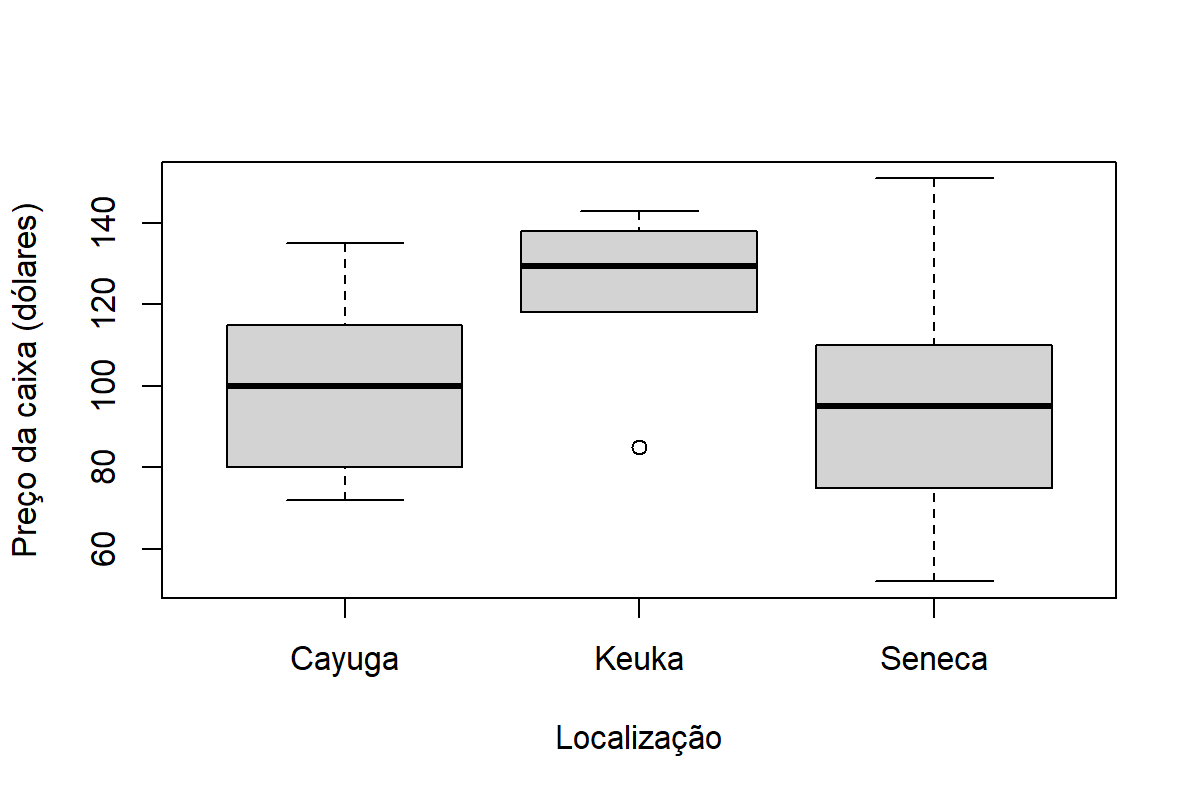
\includegraphics[width=.7\textwidth]{graficos_vinhedos}\end{center}
\begin{enumerate}[label=(\alph*)]
  \item Que tipo de gráfico é apresentado? Quais variáveis foram usadas?
  \item Qual localização produz o vinho mais caro? E o mais barato?
  \item Em qual localização os vinhos geralmente são mais caros?
  \item Descreva e compare a distribuição dos preços nas três regiões.
\end{enumerate}
\item Faça um esboço de histograma para os escores de QI de uma amostra, dados na tabela. Atenção às amplitudes das classes.
\begin{center}
\begin{tabular}{c|c}
\toprule
QI & Frequência absoluta \\
\midrule
65--69 & 2 \\ 70--84 & 16 \\ 85--99 & 34 \\ 100--114 & 37 \\ 115--129 & 11 \\ 130--144 & 3 \\
\midrule
Total & 103 \\
\bottomrule
\end{tabular}
\end{center}

\end{enumerate}

\bigskip
\needspace{12\baselineskip}
\section*{Aprofundamento: contas nacionais e dados reais}
\noindent\textit{Exercícios com dados oficiais, ligados à seção de contas nacionais do Capítulo 1 do livro.}

\begin{enumerate}[label=\textbf{A\arabic*.}, leftmargin=*]
\item \textbf{(PIB pela ótica da despesa.)} Componentes do PIB do Brasil em 2025, a preços correntes (R\$ milhões; IBGE, Contas Nacionais Trimestrais):
\begin{center}
\begin{tabular}{lr}
\toprule
Componente & R\$ milhões \\
\midrule
Consumo das famílias & 8.081.333 \\
Consumo do governo & 2.437.414 \\
Formação bruta de capital fixo (FBCF) & 2.145.050 \\
Variação de estoques & 30.186 \\
Exportações de bens e serviços & 2.270.104 \\
Importações de bens e serviços & 2.225.524 \\
\midrule
PIB & 12.738.566 \\
\bottomrule
\end{tabular}
\end{center}
\begin{enumerate}[label=(\alph*)]
  \item Classifique as variáveis ``componente'' e ``valor''.
  \item Verifique a identidade $PIB = C + G + FBCF + \Delta E + X - M$. A diferença de poucos milhões tem alguma importância? De onde ela vem?
  \item Construa uma tabela com a participação (\%) de cada componente no PIB, com as importações entrando com sinal negativo.
    Quanto somam as participações positivas?
  \item Um colega propõe um gráfico de setores (pizza) para essa tabela. Explique por que ele não é adequado e sugira um gráfico melhor.
\end{enumerate}

\item \textbf{(Contas regionais.)} PIB e população das grandes regiões em 2021 (IBGE, Contas Regionais):
\begin{center}
\begin{tabular}{lrr}
\toprule
Região & PIB (R\$ bilhões) & População (mil) \\
\midrule
Norte & 564,1 & 18.907 \\
Nordeste & 1.243,1 & 57.668 \\
Sudeste & 4.713,0 & 89.633 \\
Sul & 1.559,8 & 30.403 \\
Centro-Oeste & 932,2 & 16.707 \\
\midrule
Brasil & 9.012,1 & 213.318 \\
\bottomrule
\end{tabular}
\end{center}
{\footnotesize Os totais podem diferir da soma das parcelas por arredondamento.}

\begin{enumerate}[label=(\alph*)]
  \item Calcule a participação de cada região no PIB e na população, e o PIB \emph{per capita} de cada região e do Brasil.
  \item Qual região tem a maior diferença entre participação no PIB e participação na população? Interprete.
  \item Que gráfico você usaria para comparar, lado a lado, as duas participações? Esboce-o.
\end{enumerate}

\end{enumerate}

\end{document}
